\documentclass[9pt]{beamer}

\usepackage{algorithm}
\usepackage{algpseudocode}
\usepackage{amsfonts}
\usepackage{amsmath}
\usepackage{amssymb}
\usepackage{cuted}
\usepackage{hyperref}
\usepackage{lmodern}
\usepackage{mathtools}
\usepackage{multirow}
\usepackage{subcaption}
\usepackage{siunitx}
\usepackage[short]{optidef}

\usetheme{Boadilla}

\begin{document}

\begin{frame}{Signal and channel}
    MISO, one $L$-reflector IRS, single-user, $N$-subband
    \begin{itemize}
        \item transmit signal at antenna $m$:
        \begin{equation}\label{eq:x_m}
            x_m(t)=\Re\left\{\sum_{n=1}^N\left({w_{I,n,m}\tilde{x}_{I,n}(t)}+w_{P,n,m}\right){e^{j2{\pi}{f_n}{t}}}\right\}
        \end{equation}
        \item composite channel at subband $n$:
        \begin{itemize}
            \item AP-user direct channel $\boldsymbol{h}_{D,n}^H \in \mathbb{C}^{1 \times M}$
            \item IRS-aided extra channel: concatenate the following terms
            \begin{itemize}
                \item AP-IRS incident channel $\boldsymbol{H}_{I,n} \in \mathbb{C}^{L \times M}$
                \item IRS reflection diagonal matrix $\boldsymbol{\Theta} = \mathrm{diag}(\gamma_1 e^{j \theta_1}, \dots, \gamma_L e^{j \theta_L}) \in \mathbb{C}^{L \times L}$
                \item IRS-user reflective channel $\boldsymbol{h}_{R,n}^H \in \mathbb{C}^{1 \times L}$
            \end{itemize}
        \end{itemize}
        \begin{equation}\label{eq:h_{n}}
            \boldsymbol{h}_{n}^H = \boldsymbol{h}_{D,n}^H + \boldsymbol{h}_{R,n}^H \boldsymbol{\Theta} \boldsymbol{H}_{I,n} = \boldsymbol{h}_{D,n}^H + \alert{\boldsymbol{\phi}^H} \boldsymbol{V}_{n}
        \end{equation}
        where $\boldsymbol{\phi}=[\gamma_1 e^{j \theta_1}, \dots, \gamma_L e^{j \theta_L}]\alert{^H} \in \mathbb{C}^{L \times 1}$ and $\boldsymbol{V}_{n}=\mathrm{diag}(\boldsymbol{h}_{R,n}^H)\boldsymbol{H}_{I,n} \in \mathbb{C}^{L \times M}$.
        \item received signal
        \begin{equation}
            y(t)=\Re\left\{\sum_{n=1}^N{\boldsymbol{h}_n^H}\left({\boldsymbol{w}_{I,n}\tilde{x}_{I,n}(t)}+\boldsymbol{w}_{P,n}\right){e^{j2{\pi}{f_n}{t}}}\right\}
        \end{equation}
    \end{itemize}
\end{frame}

\begin{frame}{Problem formulation}
    \begin{maxi!}
		{\boldsymbol{w}_I,\boldsymbol{w}_P,\boldsymbol{\phi},\rho}{z(\boldsymbol{w}_I,\boldsymbol{w}_P,\boldsymbol{\phi},\rho)}{\label{op:su}}{\label{eq:su_target}}
		\addConstraint{\frac{1}{2}({\boldsymbol{w}_I^H}{\boldsymbol{w}_I}+{\boldsymbol{w}_P^H}{\boldsymbol{w}_P})\le{P}}
		\addConstraint{\sum_{n}{\log_2\left(1+\frac{(1-\rho)\lvert(\boldsymbol{h}_{D,n}^H+\boldsymbol{\phi}^H\boldsymbol{V}_n)\boldsymbol{w}_{I,n}\rvert^2}{\sigma_n^2}\right)} \ge \bar{R}}\label{eq:su_rate_constraint}
		\addConstraint{\lvert{\phi_l}\rvert=1, \quad l=1,\dots,L}
		\addConstraint{0 \le \rho \le 1}
    \end{maxi!}
    where $\boldsymbol{w}_{I/P}=[\boldsymbol{w}_{I/P,1}^T,\dots,\boldsymbol{w}_{I/P,N}^T]^T \in \mathbb{C}^{MN \times 1}$.
\end{frame}

\begin{frame}{Challenge: the fourth-order term in current expression}
    \begin{equation}
        \mathcal{A}\left\{y_{P}^4(t)\right\} = \frac{3}{8}\sum_{\substack{{n_1},{n_2},{n_3},{n_4}\\{n_1}+{n_2}={n_3}+{n_4}}}{(\boldsymbol{h}_{{n_1}}^H\boldsymbol{w}_{P,{n_1}})(\boldsymbol{h}_{{n_2}}^H\boldsymbol{w}_{P,{n_2}})(\boldsymbol{h}_{{n_3}}^H\boldsymbol{w}_{P,{n_3}})^H(\boldsymbol{h}_{{n_4}}^H\boldsymbol{w}_{P,{n_4}})^H}
    \end{equation}
    Two known approaches so far:
    \begin{block}{GP}
        \begin{equation}
            \mathcal{A}\left\{y_{P}^4(t)\right\} = \frac{3}{8}\sum_{\substack{{n_1},{n_2},{n_3},{n_4}\\{n_1}+{n_2}={n_3}+{n_4}}}{s_{P,n_1}s_{P,n_2}s_{P,n_3}s_{P,n_4} \lVert{\boldsymbol{h}_{{n_1}}}\rVert \lVert{\boldsymbol{h}_{{n_2}}}\rVert \lVert{\boldsymbol{h}_{{n_3}}}\rVert \lVert{\boldsymbol{h}_{{n_4}}}\rVert}
        \end{equation}
        where $s_{P,n}$ is real scalar.
    \end{block}
    \begin{block}{SDP}
        \begin{equation}
            \mathcal{A}\left\{y_{P}^4(t)\right\} = \frac{3}{8}\sum_{n=-N+1}^{N-1}(\boldsymbol{h}^H\boldsymbol{W}_{P,n}^*\boldsymbol{h})(\boldsymbol{h}^H\boldsymbol{W}_{P,n}^*\boldsymbol{h})^H = \frac{3}{8}\sum_{n=-N+1}^{N-1}(\boldsymbol{w}_P^H\boldsymbol{H}_{k,n}^*\boldsymbol{w}_P)(\boldsymbol{w}_P^H\boldsymbol{H}_{k,n}^*\boldsymbol{w}_P)^H
        \end{equation}
        where $\boldsymbol{h}=[\boldsymbol{h}_{1}^T,\dots,\boldsymbol{h}_{N}^T]^T \in \mathbb{C}^{MN \times 1}$, $\boldsymbol{W}_{I/P,n}$, $\boldsymbol{H}_{k,n}$ keep the $n$-th ($n=-N+1,\dots,N-1$) block diagonal and null the remaining entries.
    \end{block}
\end{frame}

\begin{frame}{GP-based approach}
    \begin{block}{Joint design of $\boldsymbol{\phi}$, $s_{I/P,n}$, $\rho$}
        GP is not applicable for $\boldsymbol{\phi}$ since its real and imaginary parts could take negative value.
    \end{block}
    \vspace{1em}
    \begin{block}{Alternating optimization of ($s_{I/P,n}$, $\rho$) and $\boldsymbol{\phi}$}
        Cannot formulate IRS design as convex problem:
        \begin{itemize}
            \item need to approximate $\lVert{\boldsymbol{h}_{{n_1}}}\rVert \lVert{\boldsymbol{h}_{{n_2}}}\rVert \lVert{\boldsymbol{h}_{{n_3}}}\rVert \lVert{\boldsymbol{h}_{{n_4}}}\rVert$
            \item even if we provide first-order approximation to the fourth-order term above, $\lVert{\cdot}\rVert$ (reduce to $\lvert{\cdot}\rvert$ for SISO) produces convex objective function
            \begin{itemize}
                \item can solve dual problem but no idea to prove zero duality gap
            \end{itemize}
        \end{itemize}
    \end{block}
\end{frame}

\begin{frame}{SDP-based approach: alternating optimization of ($\boldsymbol{w}_{I/P,n}$, $\rho$) and $\boldsymbol{\phi}$}
    IRS design problem:
    \begin{maxi!}
        {\boldsymbol{\boldsymbol{\Phi}}}{\tilde{z}(\boldsymbol{\Phi})=\mathrm{Tr}(\boldsymbol{A}\boldsymbol{\Phi})}{\label{op:irs}}{}
        \addConstraint{\sum_{n}{\log_2\left(1+\frac{(1-\rho)\mathrm{Tr}(\boldsymbol{C}_n\boldsymbol{\Phi})}{\sigma_n^2}\right)} \ge \bar{R}\label{co:rate}}
        \addConstraint{\boldsymbol{\Phi}_{l,l}=1, \quad l=1,\dots,L+1}
        \addConstraint{\boldsymbol{\Phi}\succeq{0}}
        \addConstraint{\mathrm{rank}(\boldsymbol{\Phi})=1}
    \end{maxi!}
    Despite being convex, problem \ref{op:irs} is not a standard SDP due to rate constraint \ref{co:rate}, and there is no proof that the loss from SDR would be negligible. In other words, we only obtain $\boldsymbol{\Phi}^{\star}$.
    \begin{figure}
        \centering
        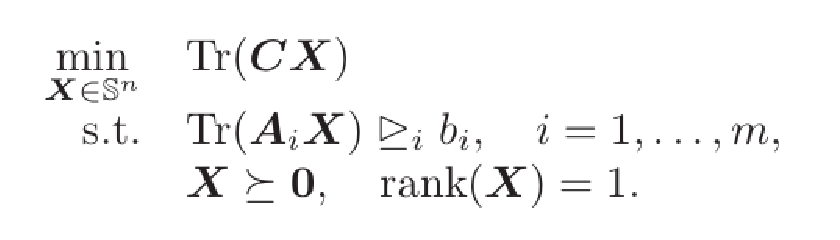
\includegraphics[width=0.5\linewidth]{assets/sdp.eps}
    \end{figure}
\end{frame}

\begin{frame}{Simulation results}
    For SISO only, simulation show that $\boldsymbol{\Phi}^{\star}$ is (always almost) rank-1, and $\boldsymbol{\phi}^{\star}$ extracted by Gaussian randomization method achieves the same performance as $\boldsymbol{\Phi}^{\star}$.
    \begin{figure}
        \centering
        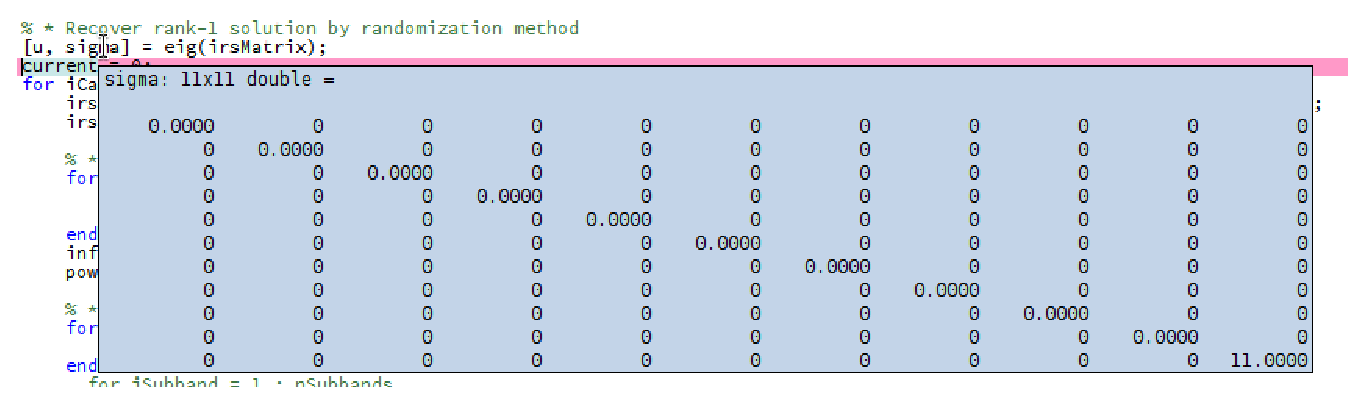
\includegraphics[width=0.8\linewidth]{assets/irs_matrix_tx_1.eps}
        \caption{Eigenvalue of $\boldsymbol{\Phi}^{\star}$ for Tx = 1}
    \end{figure}
    For MISO this is not the case.
    \begin{figure}
        \centering
        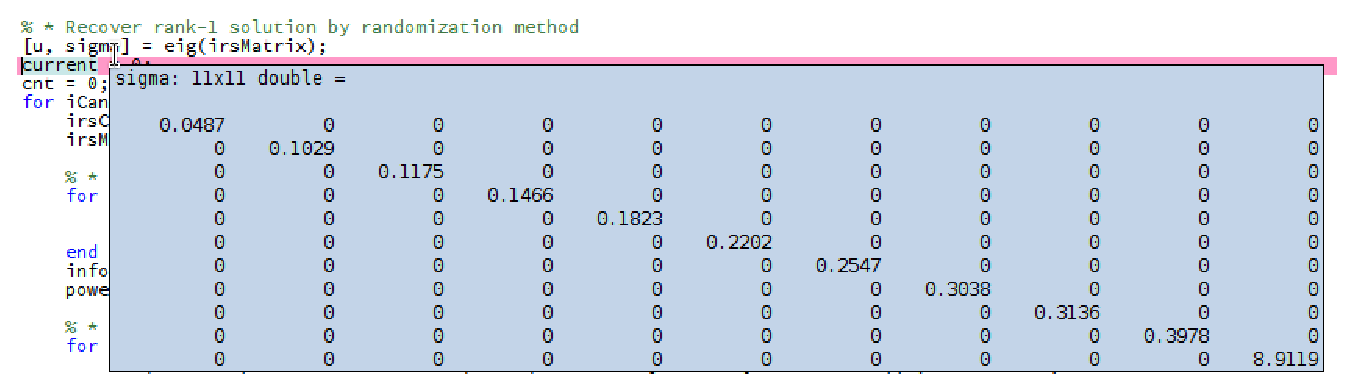
\includegraphics[width=0.8\linewidth]{assets/irs_matrix_tx_2.eps}
        \caption{Eigenvalue of $\boldsymbol{\Phi}^{\star}$ for Tx = 2}
    \end{figure}
\end{frame}

\begin{frame}{R-E plots}
    We optimize ($\boldsymbol{w}_{I/P,n}$, $\rho$) and $\boldsymbol{\phi}$ alternatively. IRS is always optimized by SDR, and the plots compare waveform optimized by GP and SDR.
    \begin{figure}[ht]
        \begin{minipage}[b]{0.5\linewidth}
            \centering
            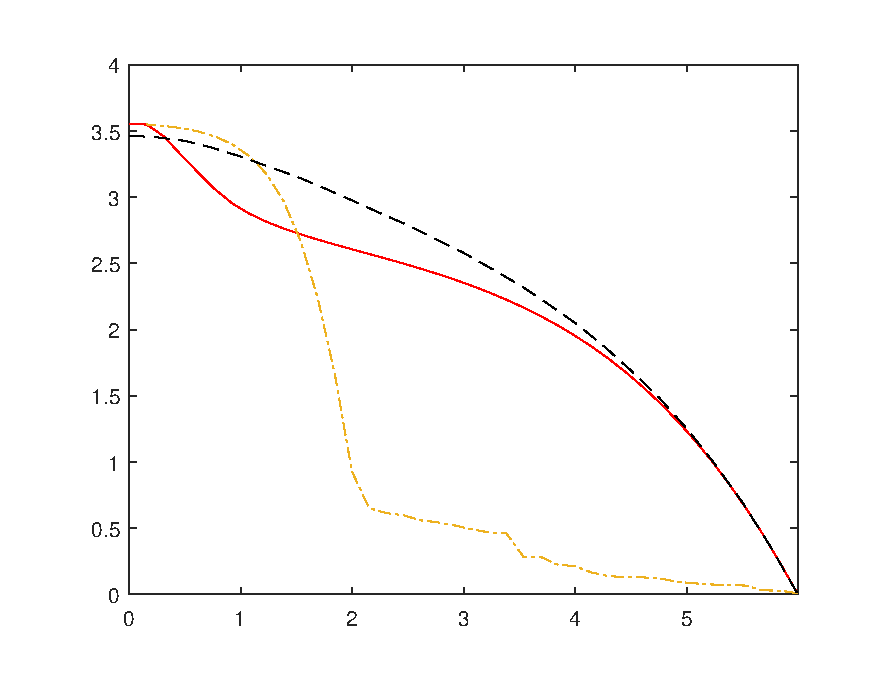
\includegraphics[width=.65\linewidth]{assets/week_29_re_gp_sdr.eps}
            \caption{GP (black) vs SDR}
            \label{fi:gp_sdr}
        \end{minipage}%
        \begin{minipage}[b]{0.5\linewidth}
            \centering
            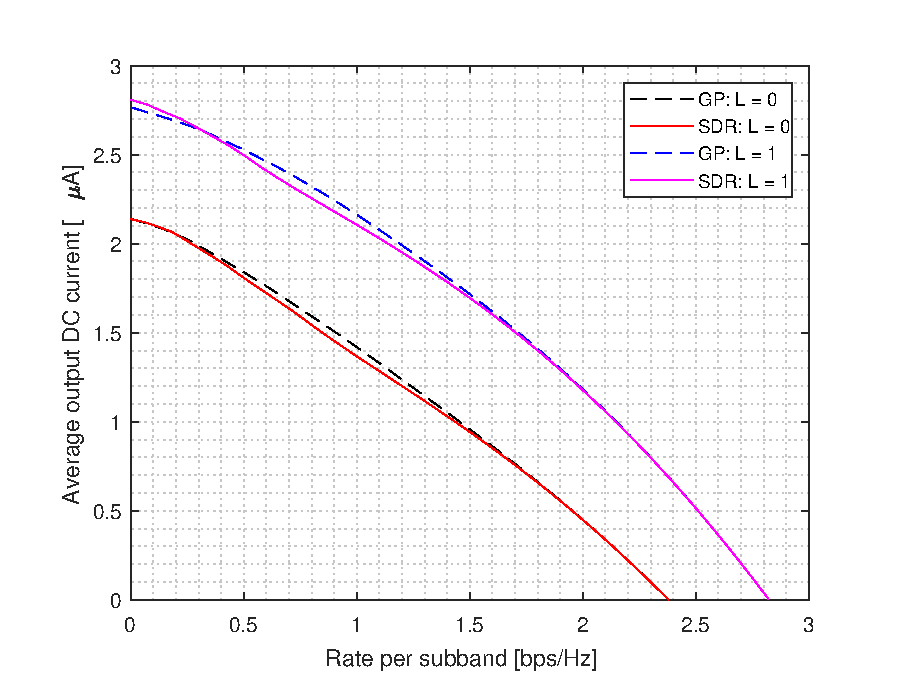
\includegraphics[width=.65\linewidth]{assets/week_29_re_irs.eps}
            \caption{No IRS vs single reflector}
        \end{minipage}
        \begin{minipage}[b]{0.5\linewidth}
            \centering
            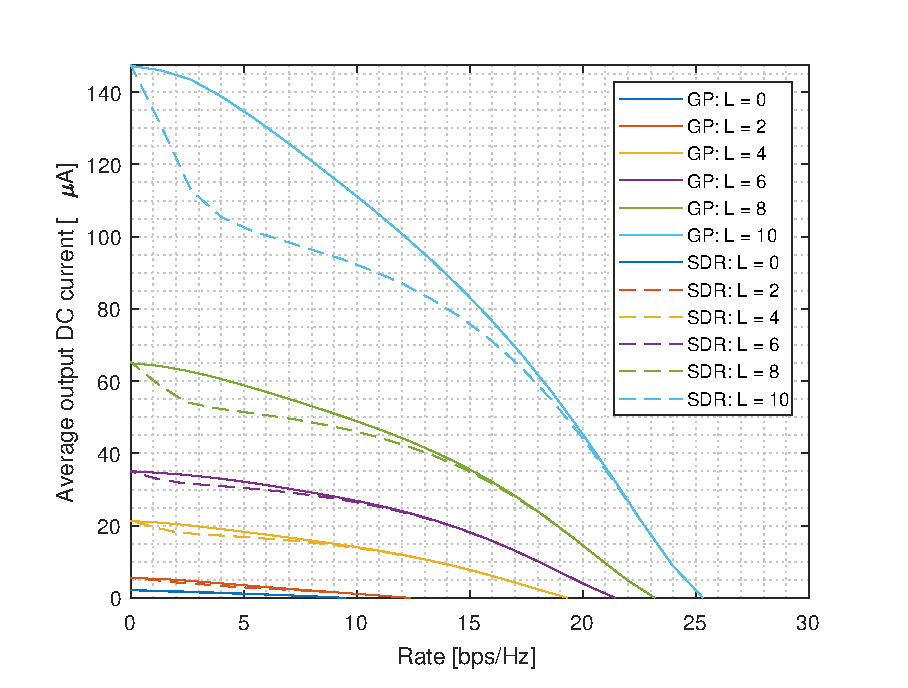
\includegraphics[width=.65\linewidth]{assets/week_29_re_reflector.eps}
            \caption{Number of reflectors}
        \end{minipage}%
        \begin{minipage}[b]{0.5\linewidth}
            \centering
            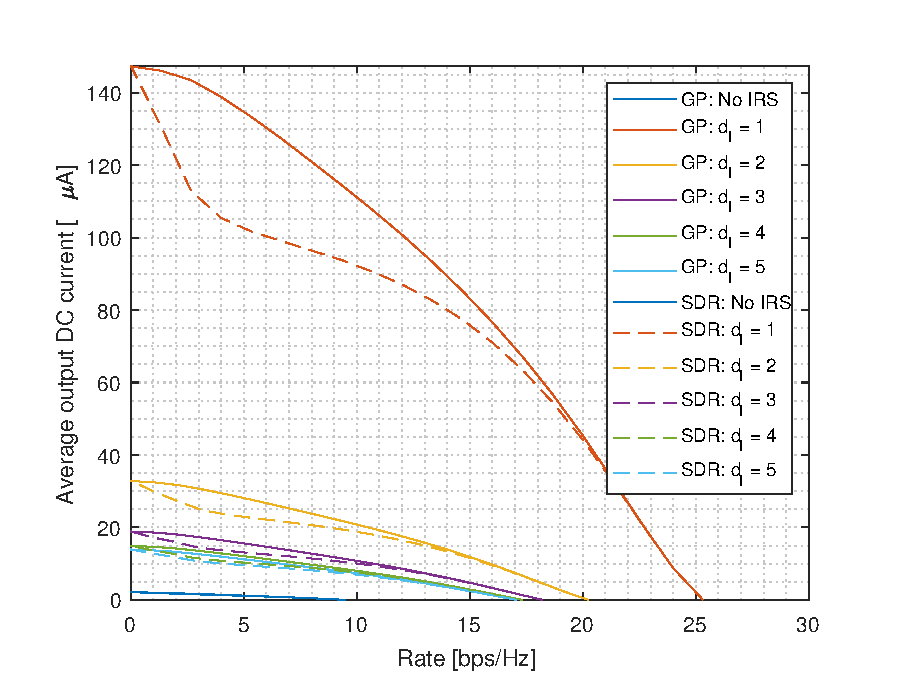
\includegraphics[width=.65\linewidth]{assets/week_29_re_distance.eps}
            \caption{AP-IRS distance}
        \end{minipage}
    \end{figure}
\end{frame}

\begin{frame}{Problem}
    \begin{itemize}
        \item Although $\boldsymbol{\Phi}^{\star}$ turns out rank-1 for SISO, we have no idea on its demonstration
        \item Even if we rewrite sum-rate constraint \ref{co:rate} as quadratic form $\mathrm{Tr}(\boldsymbol{C}\boldsymbol{\Phi})$, the approximation accuracy $\gamma$ requires further check (due to this additional constraint)
    \end{itemize}
\end{frame}

\end{document}
